\documentclass{beamer}

\usepackage{svg}
\usepackage{hyperref}
\usepackage{amsmath}
\usepackage{tikz}
\usepackage{tkz-graph}
\usepackage{pgf}
\usetikzlibrary{arrows,automata}
\usepackage{fontawesome}
\usepackage{csquotes}
\usepackage[normalem]{ulem}

\usetheme{Warsaw}
\usecolortheme{beaver}
% \usecolortheme{spruce}
\useoutertheme{infolines}
% \usetheme{Montpellier}

\title[Project introduction]{Project introduction}
\author[RJC Bilderbeek]{Rich\`{e}l JC Bilderbeek}
\institute[University of Groningen]{University of Groningen}
\date[2017-10-13]{2017-10-13}
\subject{Phylogenetics}

\AtBeginSection[]
{
  \begin{frame}
    \frametitle{Table of Contents}
    \tableofcontents[currentsection]
  \end{frame}
}

\titlegraphic{

  \href{http://github.com/richelbilderbeek/Science}{http://github.com/richelbilderbeek/Science}

  
\includegraphics[width=\textwidth,width=.18\textwidth]{rug_logo_big.png}
  \hspace*{0.05in}
  
\includegraphics[width=\textwidth,width=.50\textwidth]{gelifes-header-690x220.png}
  \hspace*{0.05in}
  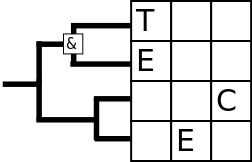
\includegraphics[width=\textwidth,width=.25\textwidth]{tece_logo_2.png}  
}

%%%%%%%%%%%%%%%%%%%%%%%%%%%%%%%%%%%%%%%%%%%%%%%%%%%%%%%%%%%%%%%%%%%%%%%%%%%%%%%%
% References
%%%%%%%%%%%%%%%%%%%%%%%%%%%%%%%%%%%%%%%%%%%%%%%%%%%%%%%%%%%%%%%%%%%%%%%%%%%%%%%%
% Don't. Add references as footnotes instead...
%%%%%%%%%%%%%%%%%%%%%%%%%%%%%%%%%%%%%%%%%%%%%%%%%%%%%%%%%%%%%%%%%%%%%%%%%%%%%%%%
\begin{document}

\frame{\titlepage}

\section[Introduction]{Introduction}

%%%%%%%%%%%%%%%%%%%%%%%%%%%%%%%%%%%%%%%%%%%%%%%%%%%%%%%%%%%%%%%%%%%%%%%%%%%%%%%%
\begin{frame}
  \frametitle{Galapagos Islands\footnotemark}

  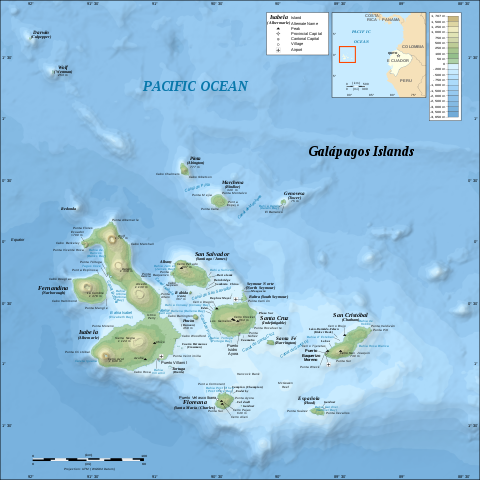
\includegraphics[height=0.7\textheight]{Galapagos_Islands_topographic_map}

  \footnotetext[1]{By: Eric Gaba (Sting - fr:Sting), translated by NordNordWest, derivative work: MatthewStevens Galapagos\_Islands\_topographic\_map-de.svg, CC BY-SA 3.0, https://commons.wikimedia.org/w/index.php?curid=16301316}

\end{frame}
%%%%%%%%%%%%%%%%%%%%%%%%%%%%%%%%%%%%%%%%%%%%%%%%%%%%%%%%%%%%%%%%%%%%%%%%%%%%%%%%


%%%%%%%%%%%%%%%%%%%%%%%%%%%%%%%%%%%%%%%%%%%%%%%%%%%%%%%%%%%%%%%%%%%%%%%%%%%%%%%%
\begin{frame}
  \frametitle{Island history\footnotemark}

  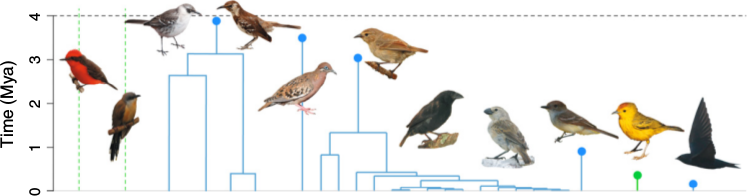
\includegraphics[width=\textwidth]{Valente_et_al_2015_fig_1.png}

  \footnotetext[1]{From Valente, Luis M., Albert B. Phillimore, and Rampal S. Etienne. "Equilibrium and non‐equilibrium dynamics simultaneously operate in the Galápagos islands." Ecology letters 18.8 (2015): 844-852.}

\end{frame}
%%%%%%%%%%%%%%%%%%%%%%%%%%%%%%%%%%%%%%%%%%%%%%%%%%%%%%%%%%%%%%%%%%%%%%%%%%%%%%%%

%%%%%%%%%%%%%%%%%%%%%%%%%%%%%%%%%%%%%%%%%%%%%%%%%%%%%%%%%%%%%%%%%%%%%%%%%%%%%%%%
\begin{frame}
  \frametitle{News\footnotemark}

  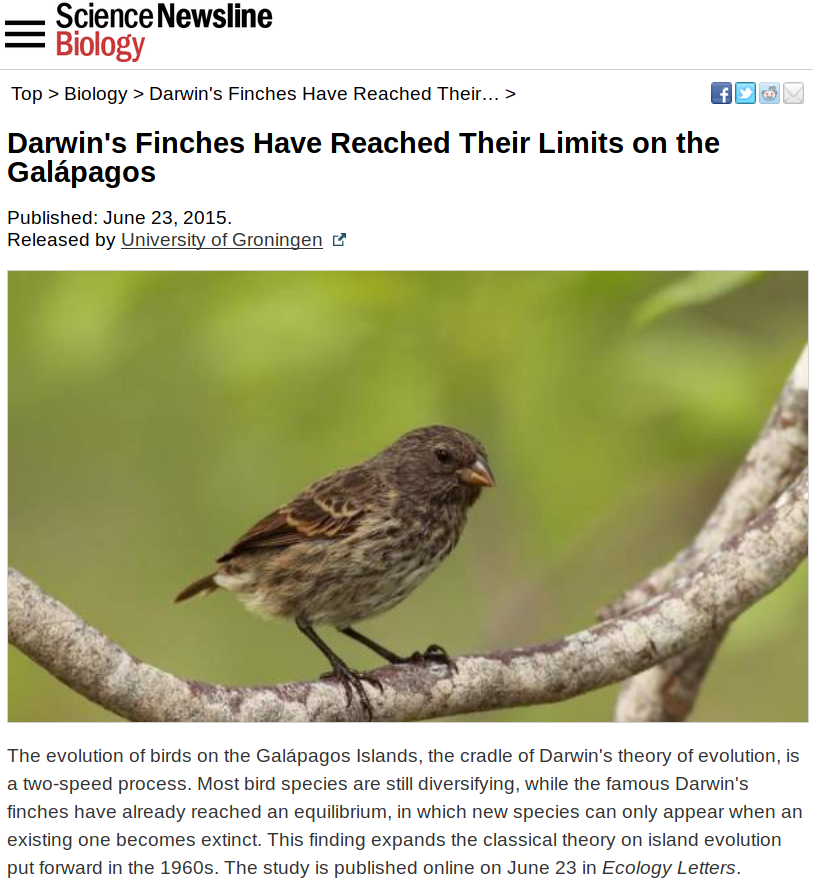
\includegraphics[height=0.8\textheight]{Press.png}

  \footnotetext[1]{http://www.sciencenewsline.com/news/2015062314370040.html}

\end{frame}
%%%%%%%%%%%%%%%%%%%%%%%%%%%%%%%%%%%%%%%%%%%%%%%%%%%%%%%%%%%%%%%%%%%%%%%%%%%%%%%%

%%%%%%%%%%%%%%%%%%%%%%%%%%%%%%%%%%%%%%%%%%%%%%%%%%%%%%%%%%%%%%%%%%%%%%%%%%%%%%%%
\begin{frame}
  \frametitle{News}

  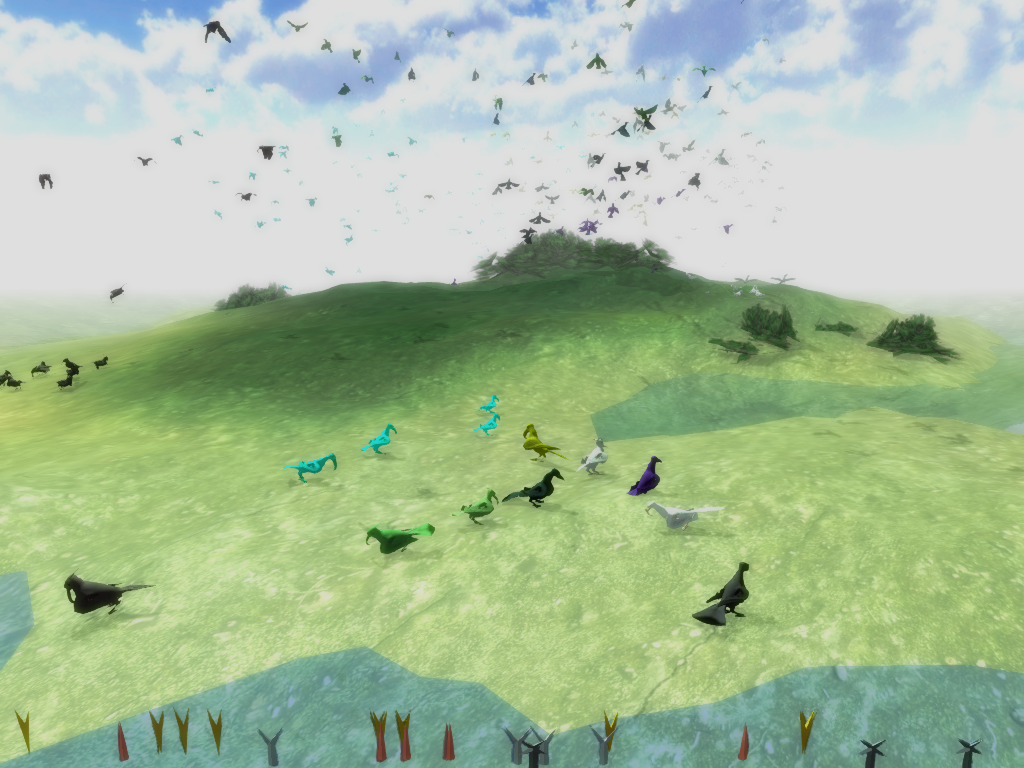
\includegraphics[height=0.8\textheight]{Finchy.png}

\end{frame}
%%%%%%%%%%%%%%%%%%%%%%%%%%%%%%%%%%%%%%%%%%%%%%%%%%%%%%%%%%%%%%%%%%%%%%%%%%%%%%%%

%%%%%%%%%%%%%%%%%%%%%%%%%%%%%%%%%%%%%%%%%%%%%%%%%%%%%%%%%%%%%%%%%%%%%%%%%%%%%%%%
\begin{frame}
  \frametitle{Caveat}

  DAISIE assumes no mainland extinction

\end{frame}
%%%%%%%%%%%%%%%%%%%%%%%%%%%%%%%%%%%%%%%%%%%%%%%%%%%%%%%%%%%%%%%%%%%%%%%%%%%%%%%%

%%%%%%%%%%%%%%%%%%%%%%%%%%%%%%%%%%%%%%%%%%%%%%%%%%%%%%%%%%%%%%%%%%%%%%%%%%%%%%%%
\begin{frame}
  \frametitle{Research question}

  What is the error DAISIE makes in parameters estimation, 
  for varying levels of mainland extinction?

\end{frame}
%%%%%%%%%%%%%%%%%%%%%%%%%%%%%%%%%%%%%%%%%%%%%%%%%%%%%%%%%%%%%%%%%%%%%%%%%%%%%%%%

%%%%%%%%%%%%%%%%%%%%%%%%%%%%%%%%%%%%%%%%%%%%%%%%%%%%%%%%%%%%%%%%%%%%%%%%%%%%%%%%
\begin{frame}
  \frametitle{What has been done?}

  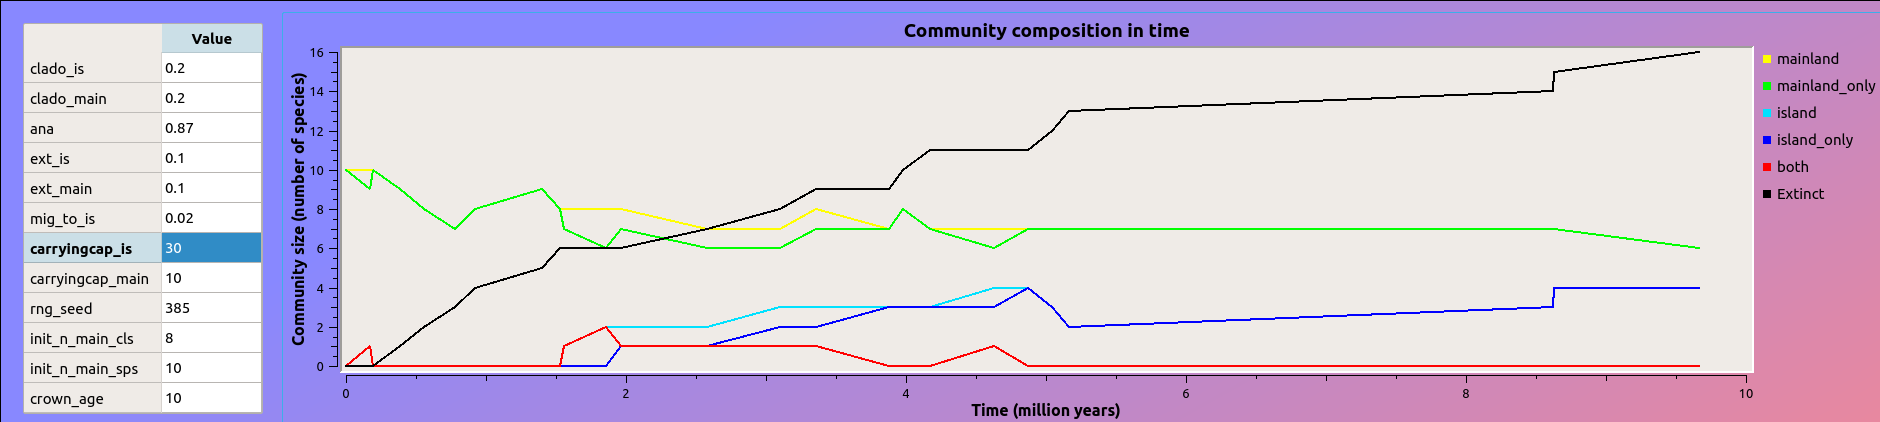
\includegraphics[width=\textwidth]{elly_top_zoom.png}

\end{frame}
%%%%%%%%%%%%%%%%%%%%%%%%%%%%%%%%%%%%%%%%%%%%%%%%%%%%%%%%%%%%%%%%%%%%%%%%%%%%%%%%

%%%%%%%%%%%%%%%%%%%%%%%%%%%%%%%%%%%%%%%%%%%%%%%%%%%%%%%%%%%%%%%%%%%%%%%%%%%%%%%%
\begin{frame}
  \frametitle{What has been done?}

  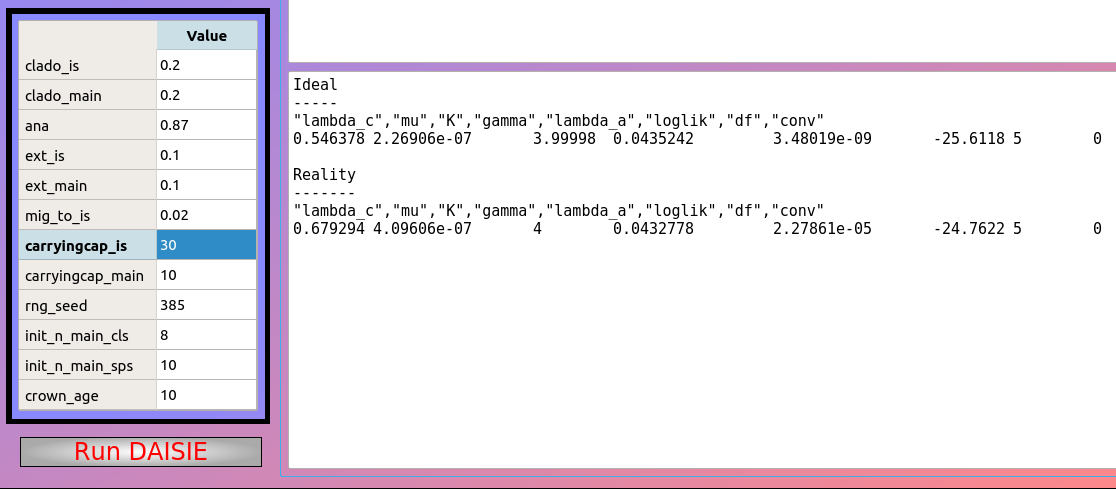
\includegraphics[width=\textwidth]{elly_bottom_zoom.png}

\end{frame}
%%%%%%%%%%%%%%%%%%%%%%%%%%%%%%%%%%%%%%%%%%%%%%%%%%%%%%%%%%%%%%%%%%%%%%%%%%%%%%%%


%%%%%%%%%%%%%%%%%%%%%%%%%%%%%%%%%%%%%%%%%%%%%%%%%%%%%%%%%%%%%%%%%%%%%%%%%%%%%%%%
\begin{frame}
  \frametitle{What still needs to be done?}

  \begin{itemize}
    \item setup an analysis
    \item run simulations
    \item write article
    \item fix potenential flaws in current setup
  \end{itemize}

\end{frame}
%%%%%%%%%%%%%%%%%%%%%%%%%%%%%%%%%%%%%%%%%%%%%%%%%%%%%%%%%%%%%%%%%%%%%%%%%%%%%%%%

%%%%%%%%%%%%%%%%%%%%%%%%%%%%%%%%%%%%%%%%%%%%%%%%%%%%%%%%%%%%%%%%%%%%%%%%%%%%%%%%
\begin{frame}
  \frametitle{My favorite planning}

  \begin{itemize}
    \item January: Setup and run analysis. Write abstract, introduction, methods
    \item February and March: Analyse results. Write results, conclusion, discussion
  \end{itemize}

\end{frame}
%%%%%%%%%%%%%%%%%%%%%%%%%%%%%%%%%%%%%%%%%%%%%%%%%%%%%%%%%%%%%%%%%%%%%%%%%%%%%%%%


%%%%%%%%%%%%%%%%%%%%%%%%%%%%%%%%%%%%%%%%%%%%%%%%%%%%%%%%%%%%%%%%%%%%%%%%%%%%%%%%
\begin{frame}
  \frametitle{Thanks}
  
  \center
  \Huge
  \faSmileO THANKS! \faSmileO

\end{frame}
%%%%%%%%%%%%%%%%%%%%%%%%%%%%%%%%%%%%%%%%%%%%%%%%%%%%%%%%%%%%%%%%%%%%%%%%%%%%%%%%


\end{document}